\documentclass{standalone}
\usepackage{tikz}
\usepackage{ctex,siunitx}
\setCJKmainfont{Noto Serif CJK SC}
\usepackage{tkz-euclide}
\usepackage{amsmath}
\usetikzlibrary{patterns, calc,3d}
\usetikzlibrary {decorations.pathmorphing,decorations.pathreplacing,decorations.shapes}
\begin{document}
\small
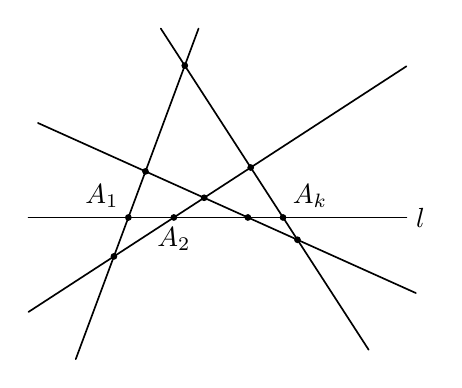
\begin{tikzpicture}[>=latex,scale=1.2]
  \tkzDefPoints{4/0/l,0/0/l',0.5/-1.5/M,1.8/2/M',0/-1/N,4/1.6/N',0.1/1.0/P,4.1/-0.8/P',1.4/2/Q,3.6/-1.4/Q'}
  \tkzInterLL(l,l')(M,M')\tkzGetPoint{A1}
  \tkzInterLL(l,l')(N,N')\tkzGetPoint{A2}
  \tkzInterLL(l,l')(P,P')\tkzGetPoint{A3}
  \tkzInterLL(l,l')(Q,Q')\tkzGetPoint{Ak}
  \tkzInterLL(P,P')(Q,Q')\tkzGetPoint{B}
  \tkzInterLL(N,N')(Q,Q')\tkzGetPoint{C}
  \tkzInterLL(M,M')(Q,Q')\tkzGetPoint{D}
  \tkzInterLL(M,M')(P,P')\tkzGetPoint{E}
  \tkzInterLL(M,M')(N,N')\tkzGetPoint{F}
  \tkzInterLL(P,P')(N,N')\tkzGetPoint{G}
  \tkzDrawSegments[semithick](M,M' l,l' N,N' P,P' Q,Q')
  \tkzDrawPoints[fill=black](A1,A2,A3,Ak,B,C,D,E,F,G)
  \tkzLabelPoints[right](l)
  \tkzLabelPoint[above left](A1){$A_1$}
  \tkzLabelPoint[below](A2){$A_2$}
  \tkzLabelPoint[above right](Ak){$A_k$}
\end{tikzpicture}
\end{document}